\subsection{System Engineering \label{sec:sysen}}
System engineering is a comprehensive and multifaceted methodology that encompasses the conceptualization, execution, and administration of intricate systems over their entire lifespan \cite{haberfellner2019systems} (see \textbf{Figure \ref{fig:v-model}}). It embraces a holistic perspective that takes into account the interactions and interdependencies between different components to achieve optimal performance and functionality. It encompasses work procedures, optimization techniques, and risk management tools in projects, ensuring comprehensive consideration and integration of all potential components of a project or system. In the context of the automotive industry, where complex systems and simulations play a central role, the application of systems engineering principles is becoming essential \cite{d2017systems}.

\subsubsection{Core Concepts}
    The key principles of systems engineering are as follows:
    \begin{itemize}
      \item \textbf{Requirements engineering}: this phase consists of determining and documenting the needs and constraints that the system must satisfy \cite{loper2015modeling}. In the context of simulation configuration, understanding requirements is crucial to accurately model and simulate real-world automotive scenarios \cite{keating2008system}.
      
      \item \textbf{System design}: this phase involves transforming the requirements into a system plan \cite{loper2015modeling, nielsen2015systems}. It involves assigning functions to components, taking into account factors such as efficiency, reliability, and maintainability. For simulation configuration, this step is essential to create a framework that aligns with the specific attributes of automotive simulations.
      
      \item \textbf{Integration and testing}: Systems engineering emphasizes the importance of rigorous testing and integration to ensure that all components work perfectly together \cite{loper2015modeling}. This is particularly relevant in the context of simulation configuration, where the accuracy and reliability of results depend on the effective integration of different simulation parameters.
      
      \item \textbf{Lifecycle management}: Systems engineering goes beyond the initial design and implementation phases \cite{loper2015modeling}. It involves continuous monitoring, maintenance, and adaptation to changing requirements throughout the system's lifecycle. This perspective is crucial to the longevity and adaptability of simulation configurations in the dynamic automotive landscape \cite{nielsen2015systems}.
    \end{itemize}

    
\subsubsection{V-Model}
The V-model illustrates systems development by highlighting the verification and validation stages \cite{clark2009system}. A graphical representation of this model is shown in \textbf{Figure \ref{fig:v-model}}. The system specification and detailed software design are presented on the left-hand side of the “V”, along with the steps leading to implementation. The steps mentioned on the left-hand side must be verified and validated on the right-hand side of the \textbf{“V”}. It also includes the integration of systems and software. Each step on the left is directly linked to a test step. Once the first stage has been successfully completed, the next stage begins.\\

\begin{figure}[H]
    \centering
    \frame{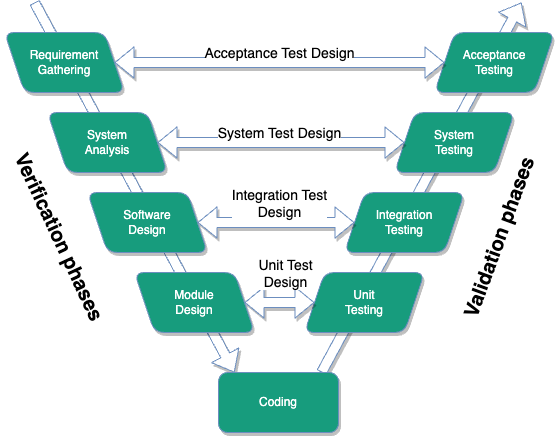
\includegraphics[scale=0.55]{images/V-Model.png}}
    \caption[V-Model]{\label{fig:v-model} V-Model \cite{clark2009system} }
\end{figure}

With the evolution of technology, many software applications exist to cover these different stages more effectively \cite{johansson1999v}. 